\begin{minipage}{\textwidth}
    \setlength{\parindent}{2em}
    To clarify each workflow, the following sequence diagrams are constructed based on the use case diagrams, in order to describe in detail the interaction process between components throughout the entire system.
\end{minipage}

% MARK STUDENT PRESENCE
\subsubsection{Sequence Diagram for Mark Student Attendance}
\vspace{-1.5em}
\begin{figure}[H]
    \centering
    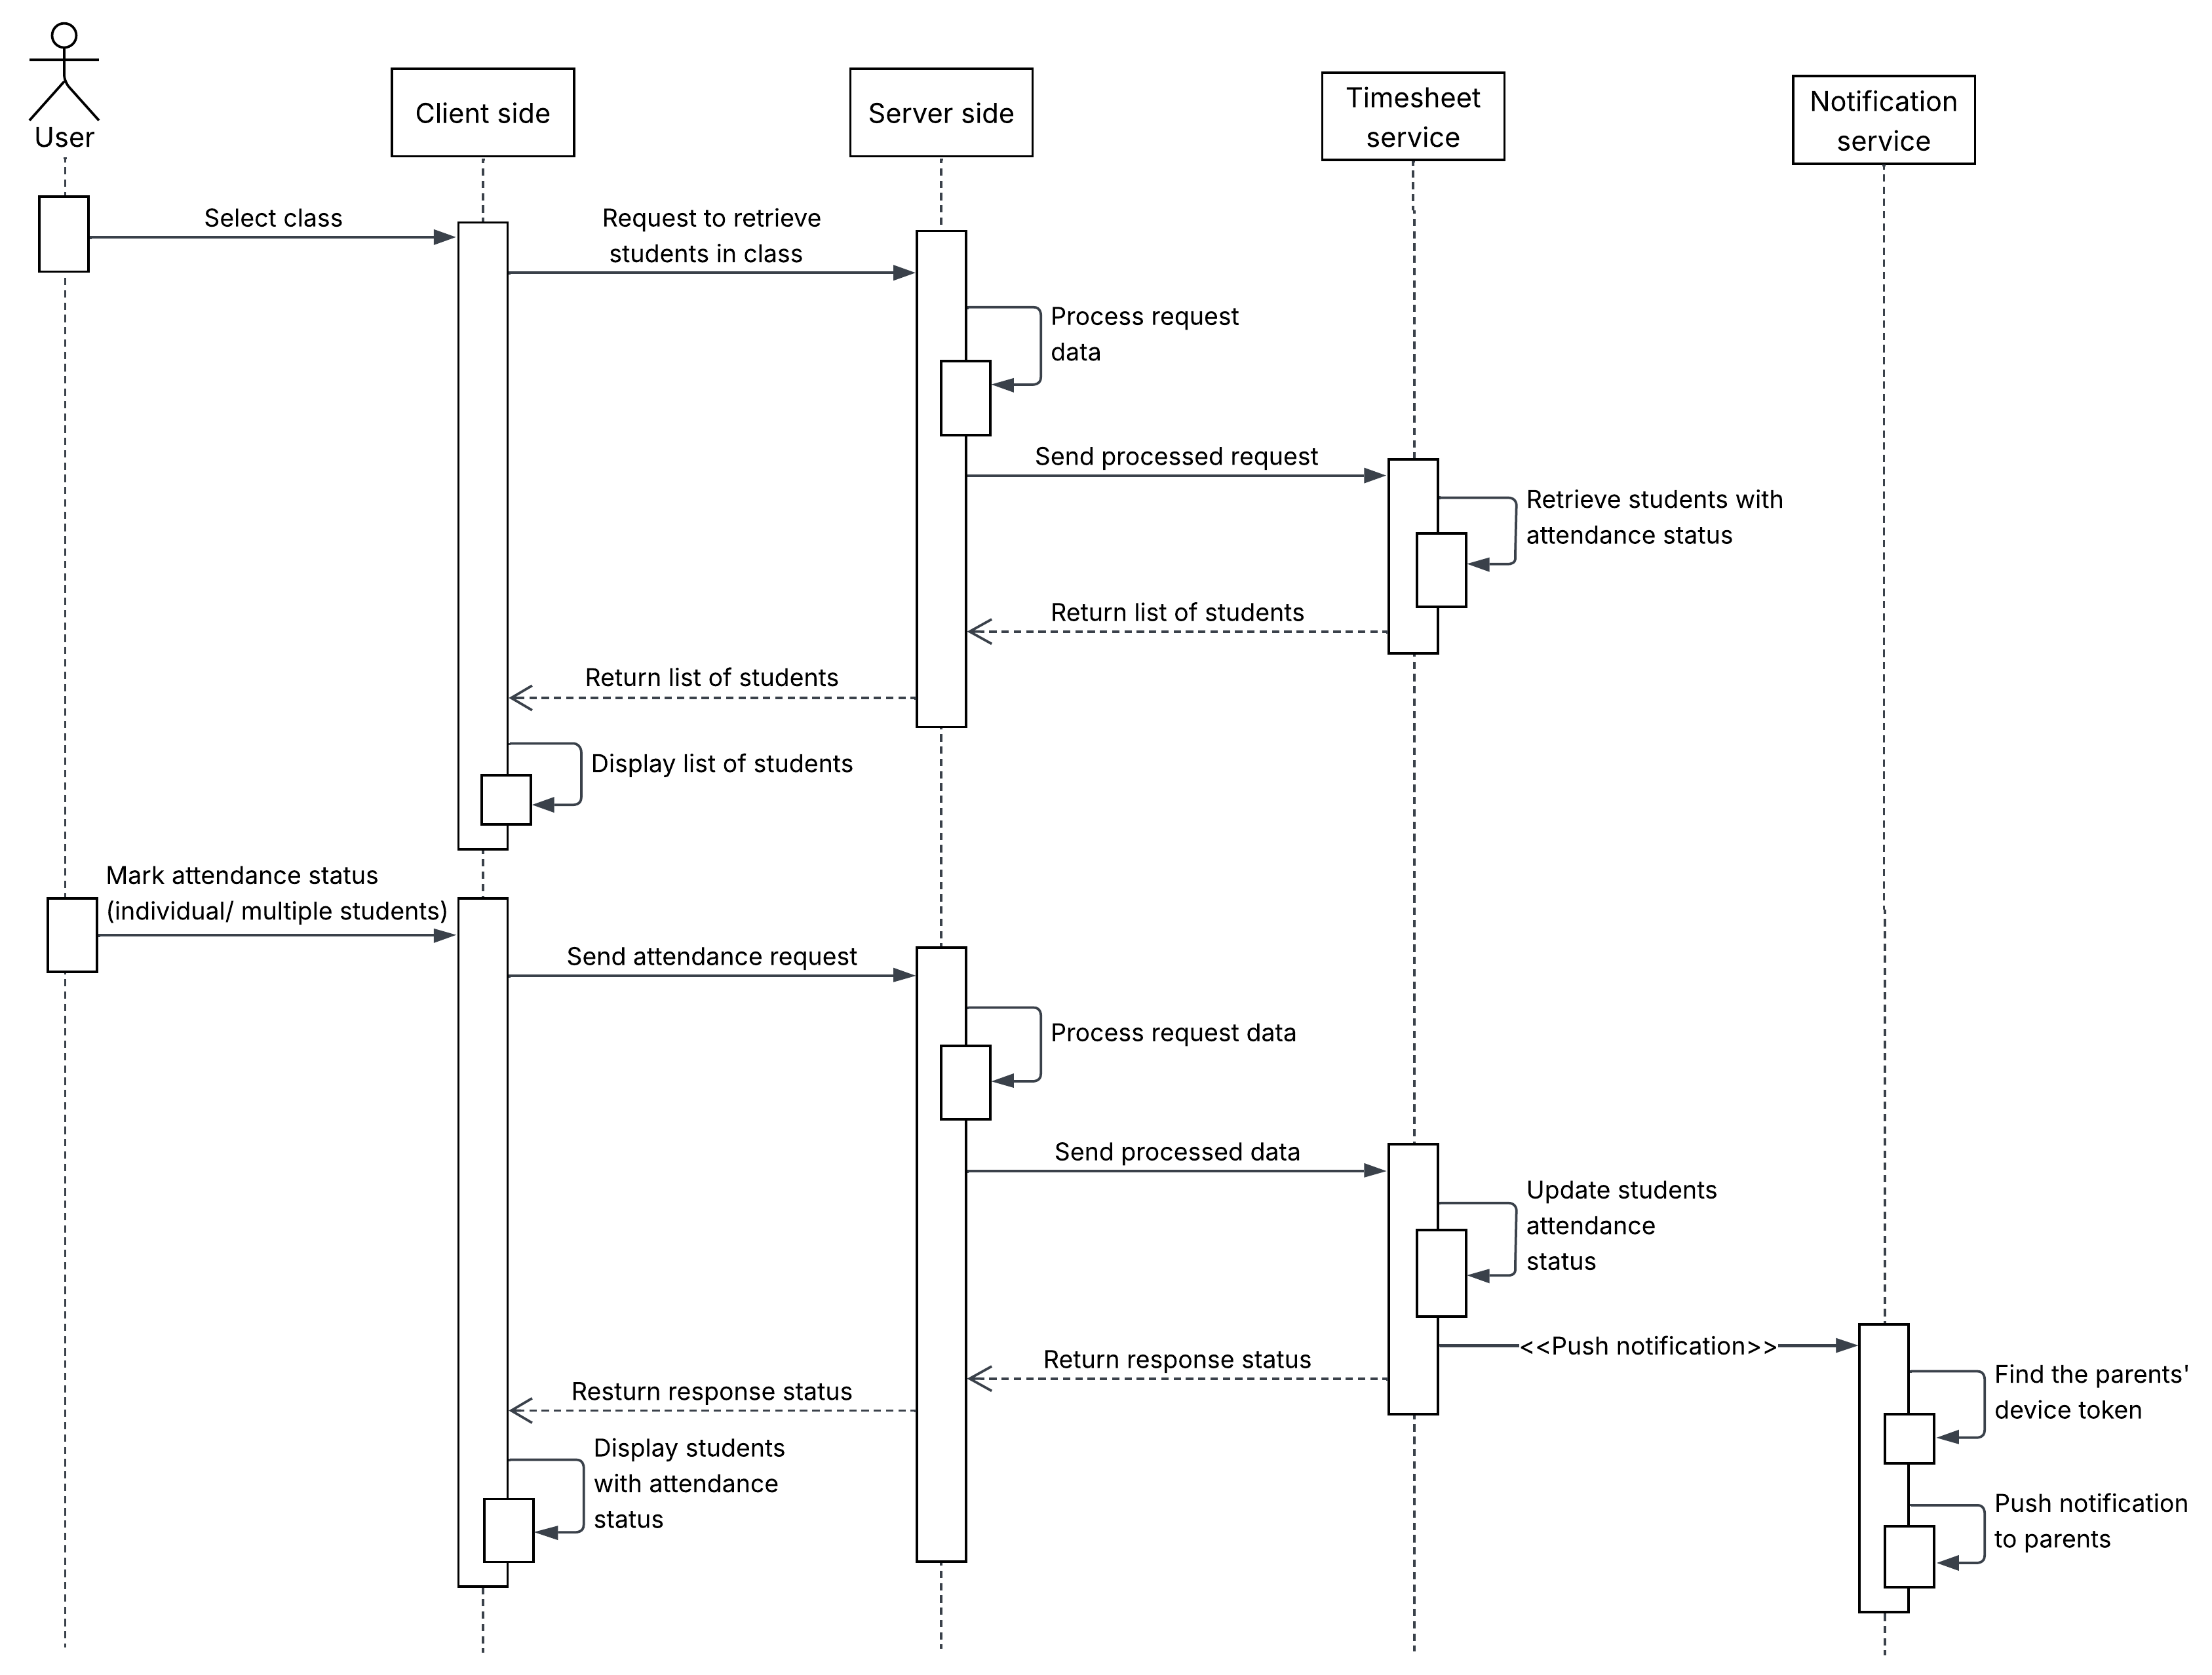
\includegraphics[width=1\textwidth]{images/sqd_mark_attendance_class.png}
    \vspace{-1em}
    \caption{Mark student presence sequence diagram.}
    \label{fig:sequence_diagram_mark_student_presence}
\end{figure}
\begin{minipage}{\textwidth}
    \setlength{\parindent}{2em}
    The sequence diagram illustrates a detailed process for marking student attendance in a classroom. When a user requests to mark attendance, the system retrieves a list of students in the class with their current attendance status (not marked, attended, absent, late, or left early). Users can update attendance records by marking individual students or multiple students simultaneously as present, absent, on excused leave, or having departed early. Once the attendance records are updated, the server asynchronously pushes notifications to parents.  
\end{minipage}

% IMPORT EMPLOYEE DATA
\subsubsection{Sequence Diagram for Import Employee Data}
\vspace{-1.5em}
\begin{figure}[H]
    \centering
    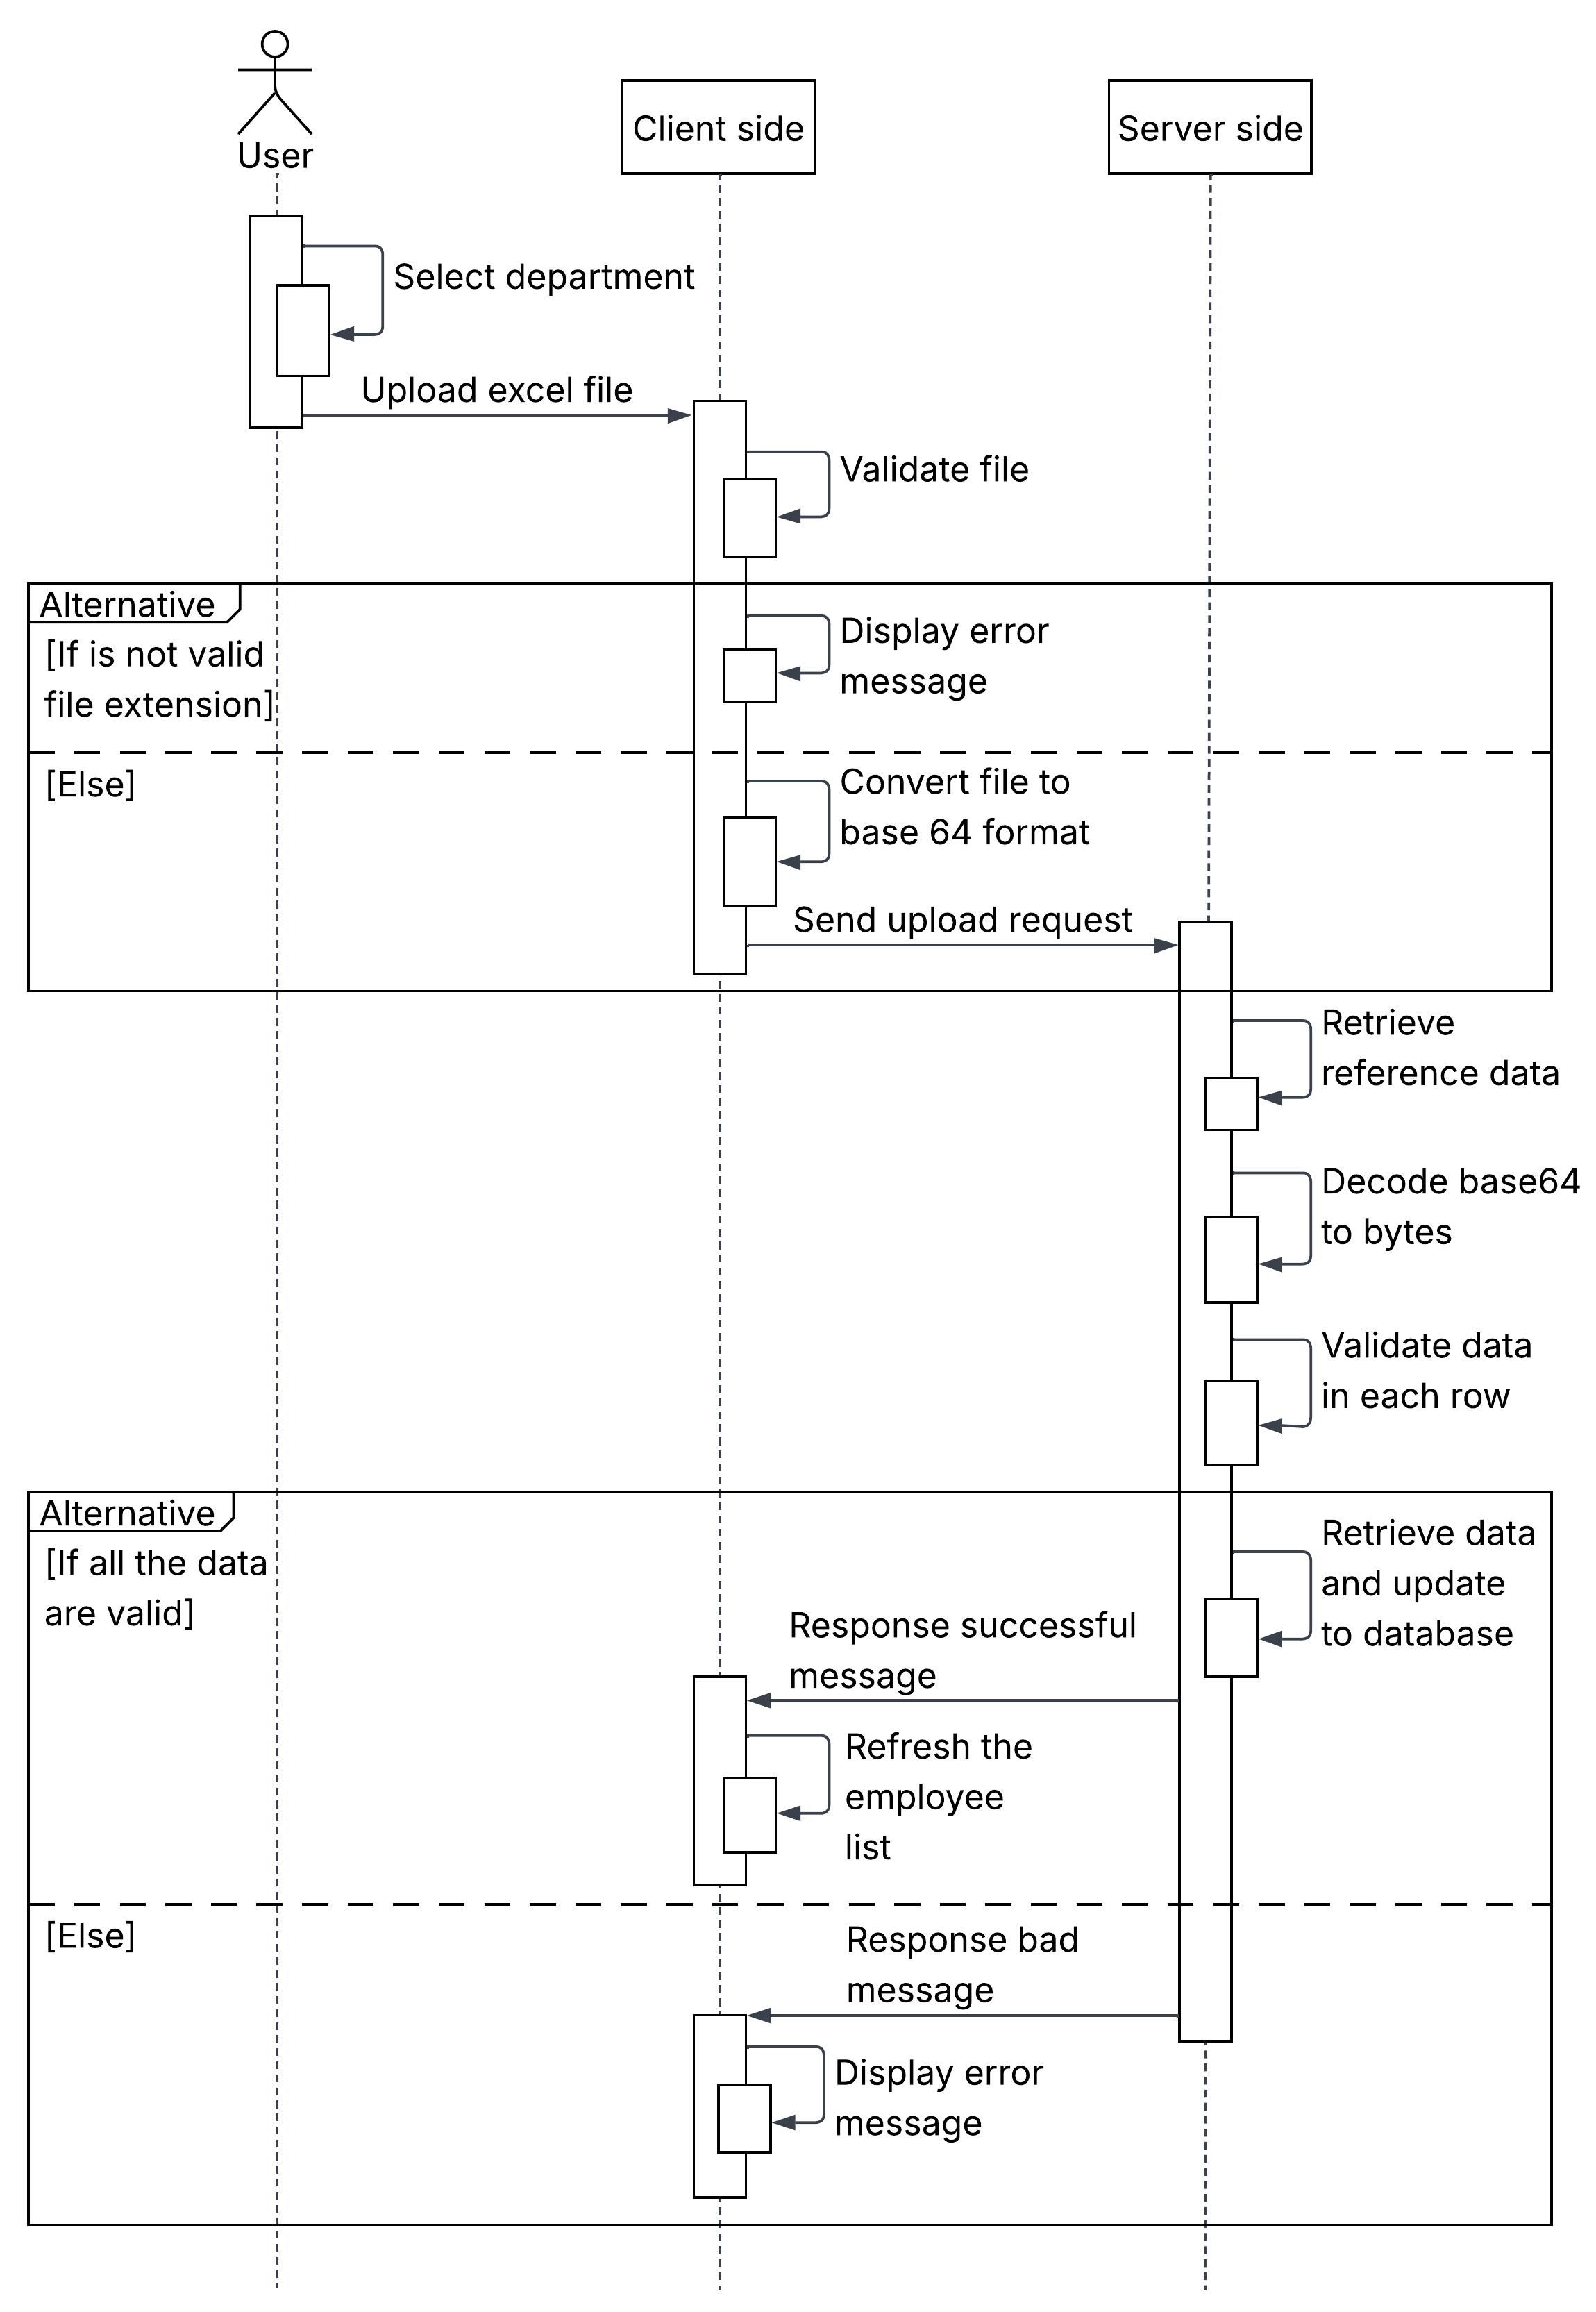
\includegraphics[width=0.8\textwidth]{images/sqd_import_employee_data.png}
    \vspace{-1em}
    \caption{Import employee data sequence diagram.}
    \label{fig:sequence_diagram_import_employee_data}
\end{figure}
\begin{minipage}{\textwidth}
    \setlength{\parindent}{2em}
    The sequence diagram illustrates a detailed process for importing employee data into the system. The user selects the department and uploads an employee Excel file. The client-side validates the format of the uploaded file. If the file format is invalid, it displays an error message to the user. Otherwise, it encodes the file to base64 format and sends a request to the server side. The server retrieves necessary reference data, decodes the file into bytes, and reads the content. The server then validates each row of data individually. If all the data is valid, the systems update the data to the database. However, if any data is invalid, it responds bad message to the user.
\end{minipage}

% CREATE LEAVE REQUEST
\subsubsection{Sequence Diagram for Create Student Leave Request}
\vspace{-1.5em}
\begin{figure}[H]
    \centering
    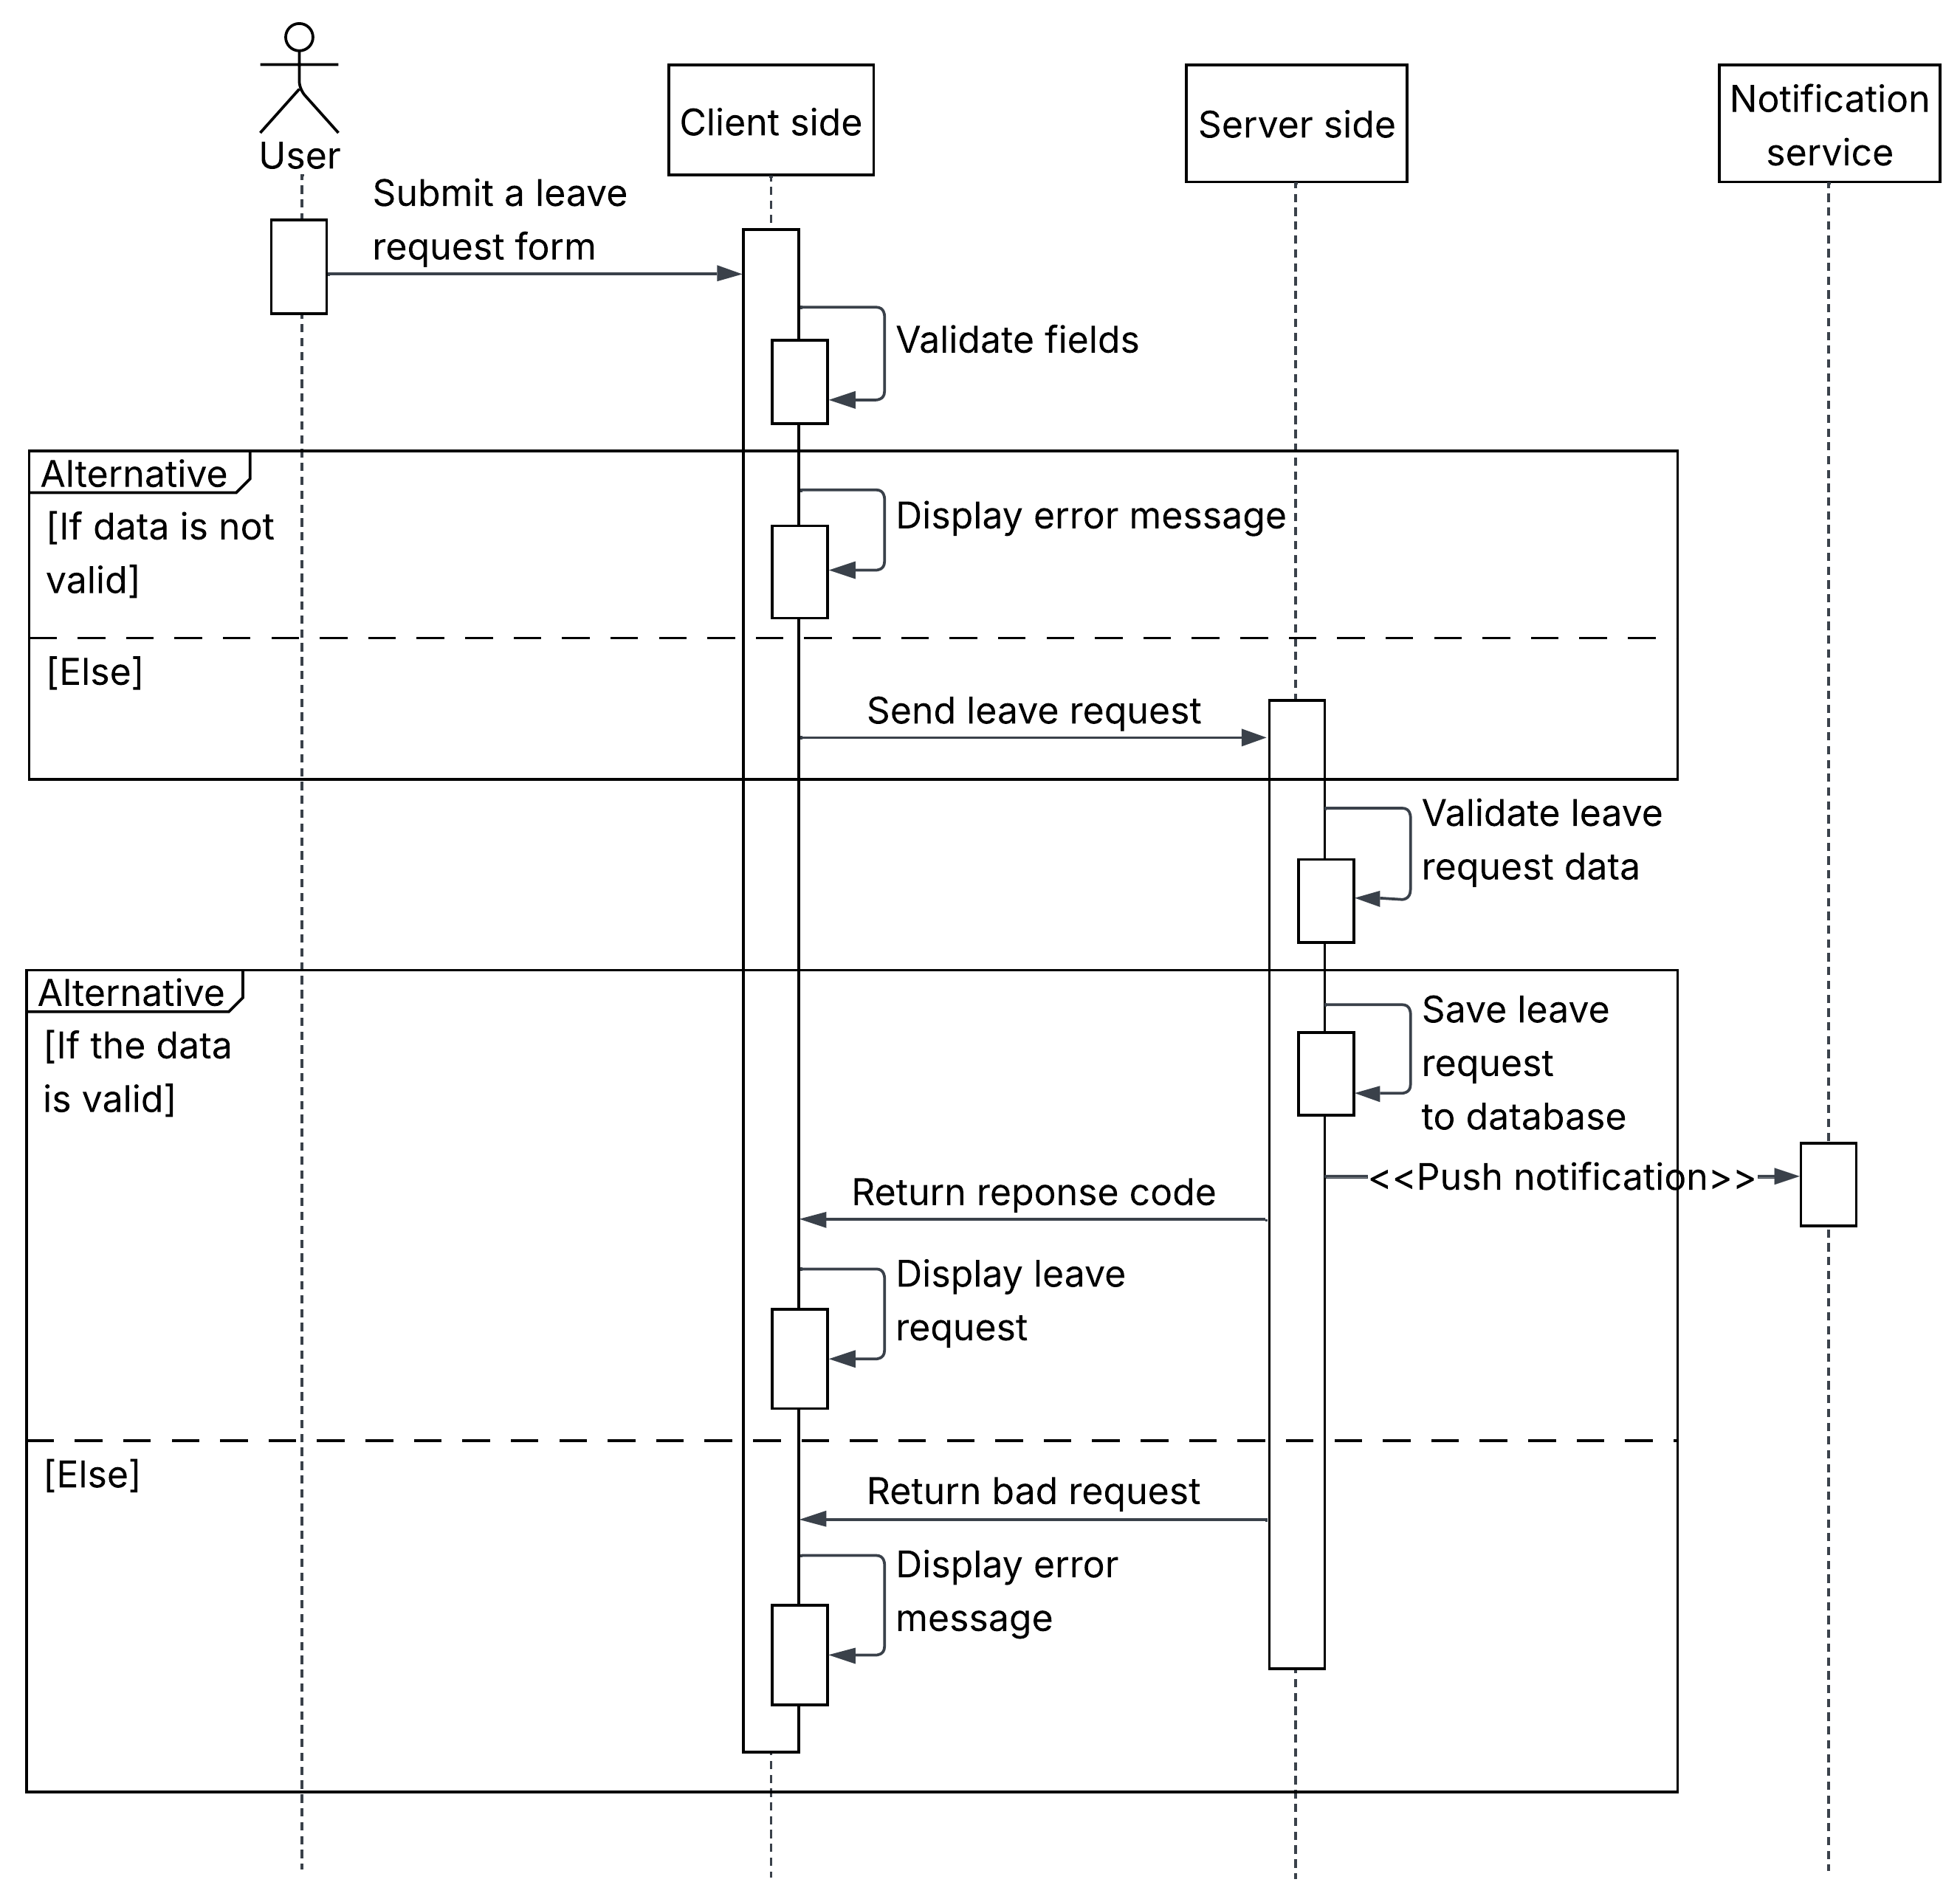
\includegraphics[width=1\textwidth]{images/sqd_create_student_leave_request.png}
    \vspace{-1em}
    \caption{Create student leave request sequence diagram.}
    \label{fig:sequence_diagram_create_student_leave_request}
\end{figure}
\begin{minipage}{\textwidth}
    \setlength{\parindent}{2em}
    The sequence diagram illustrates the operation when parents create a leave request for their child. First, they fill in all the required fields in the forms. The system checks these fields on the client side to make sure the information is valid. If everything is correct, the request is sent to the server. On the server side, the system performs further checks to prevent duplicate requests, such as overlapping dates or requests during holidays. Once the request passes all validations, it is saved to the database, and a notification is sent to the teacher. This process helps parents efficiently submit and track leave requests while ensuring teachers are promptly informed of planned student absences.
\end{minipage}

% CONFIRM LEAVE REQUEST
\subsubsection{Sequence Diagram for Confirm Student Leave Request}
\vspace{-1.5em}
\begin{figure}[H]
    \centering
    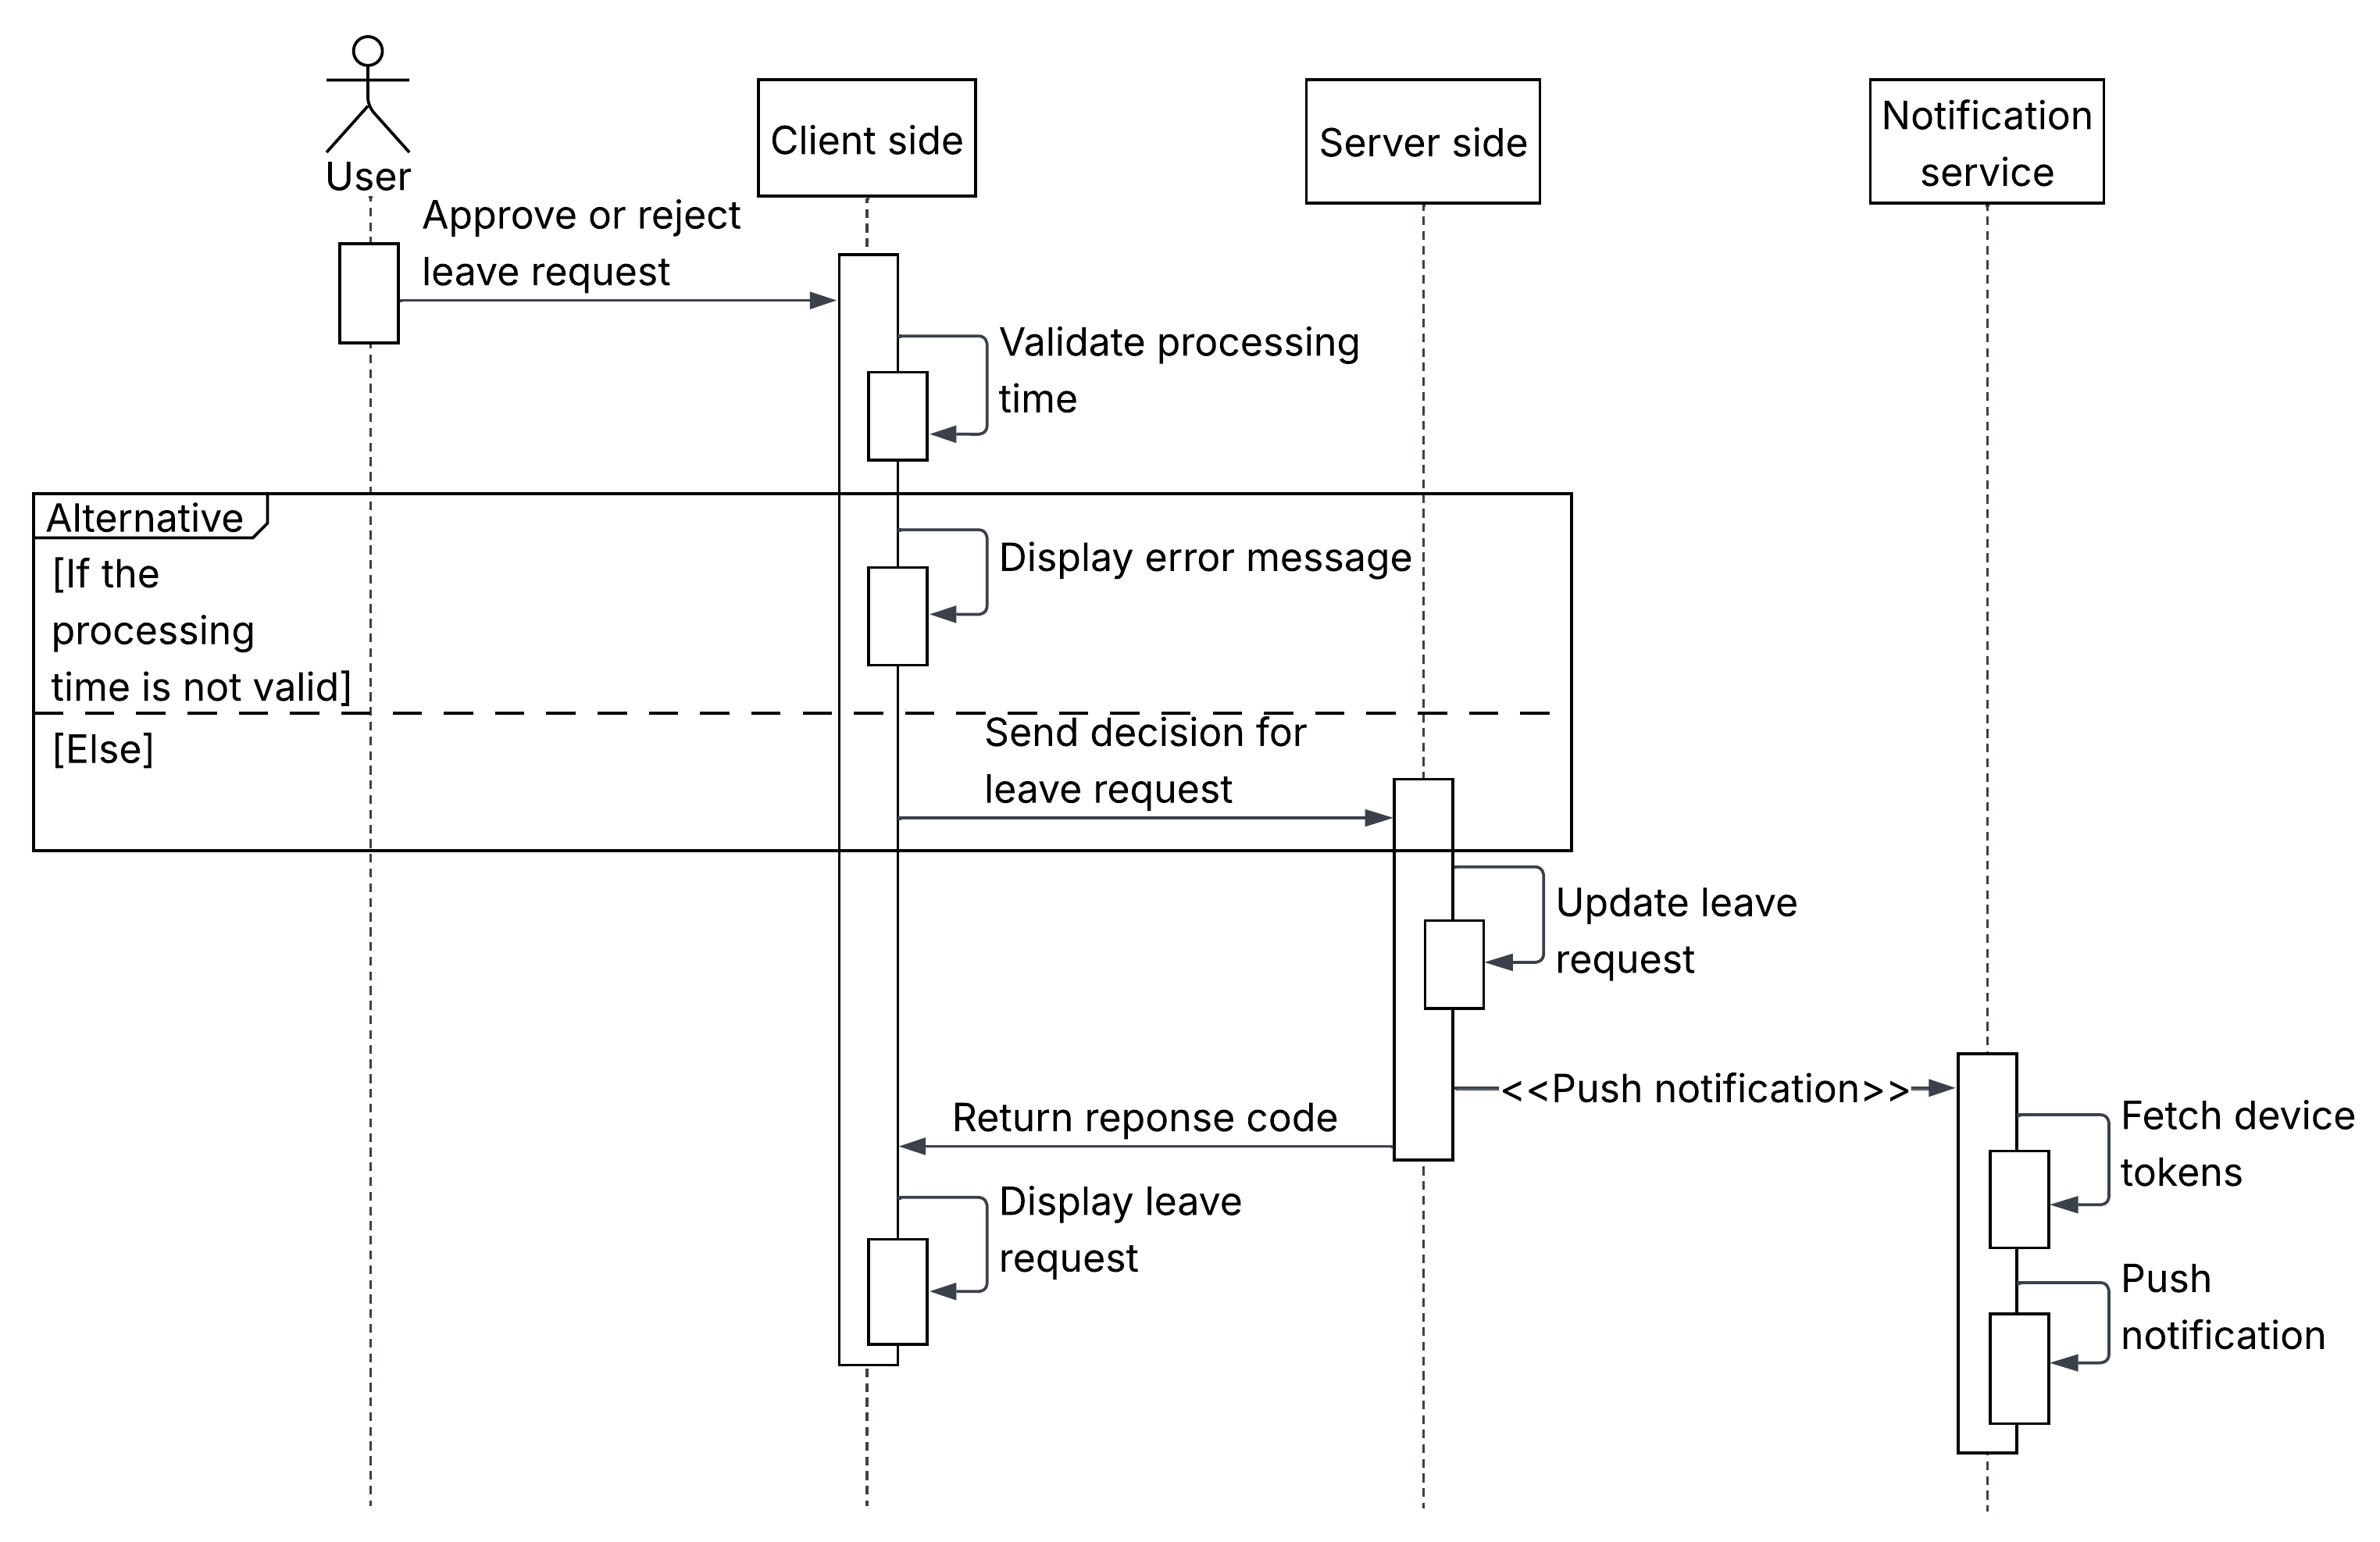
\includegraphics[width=1\textwidth]{images/sqd_confirm_student_leave_request.png}
    \vspace{-1em}
    \caption{Confirm student leave request sequence diagram.}
    \label{fig:sequence_diagram_confirm_student_leave_request}
\end{figure}
\begin{minipage}{\textwidth}
    \setlength{\parindent}{2em}
    The sequence diagram illustrates the operation when teachers confirm or reject student leave requests. First, the client side checks the date range of the leave request. If the confirmation date is after or outside the leave request date range, teachers cannot confirm or reject the request. Otherwise, they can proceed with their decision. Next, the decision for the leave request is sent to the server, which updates the leave request status, records the confirming teacher's information, and pushes notifications to parents. Once the process is successful, parents can view the updated leave request status. This process makes it easier for teachers to quickly review and approve student leave requests, with all details properly recorded.
\end{minipage}

% CREATE NEWSFEED POST
\subsubsection{Sequence Diagram for Post Newsfeed}
\vspace{-1.5em}
\begin{figure}[H]
    \centering
    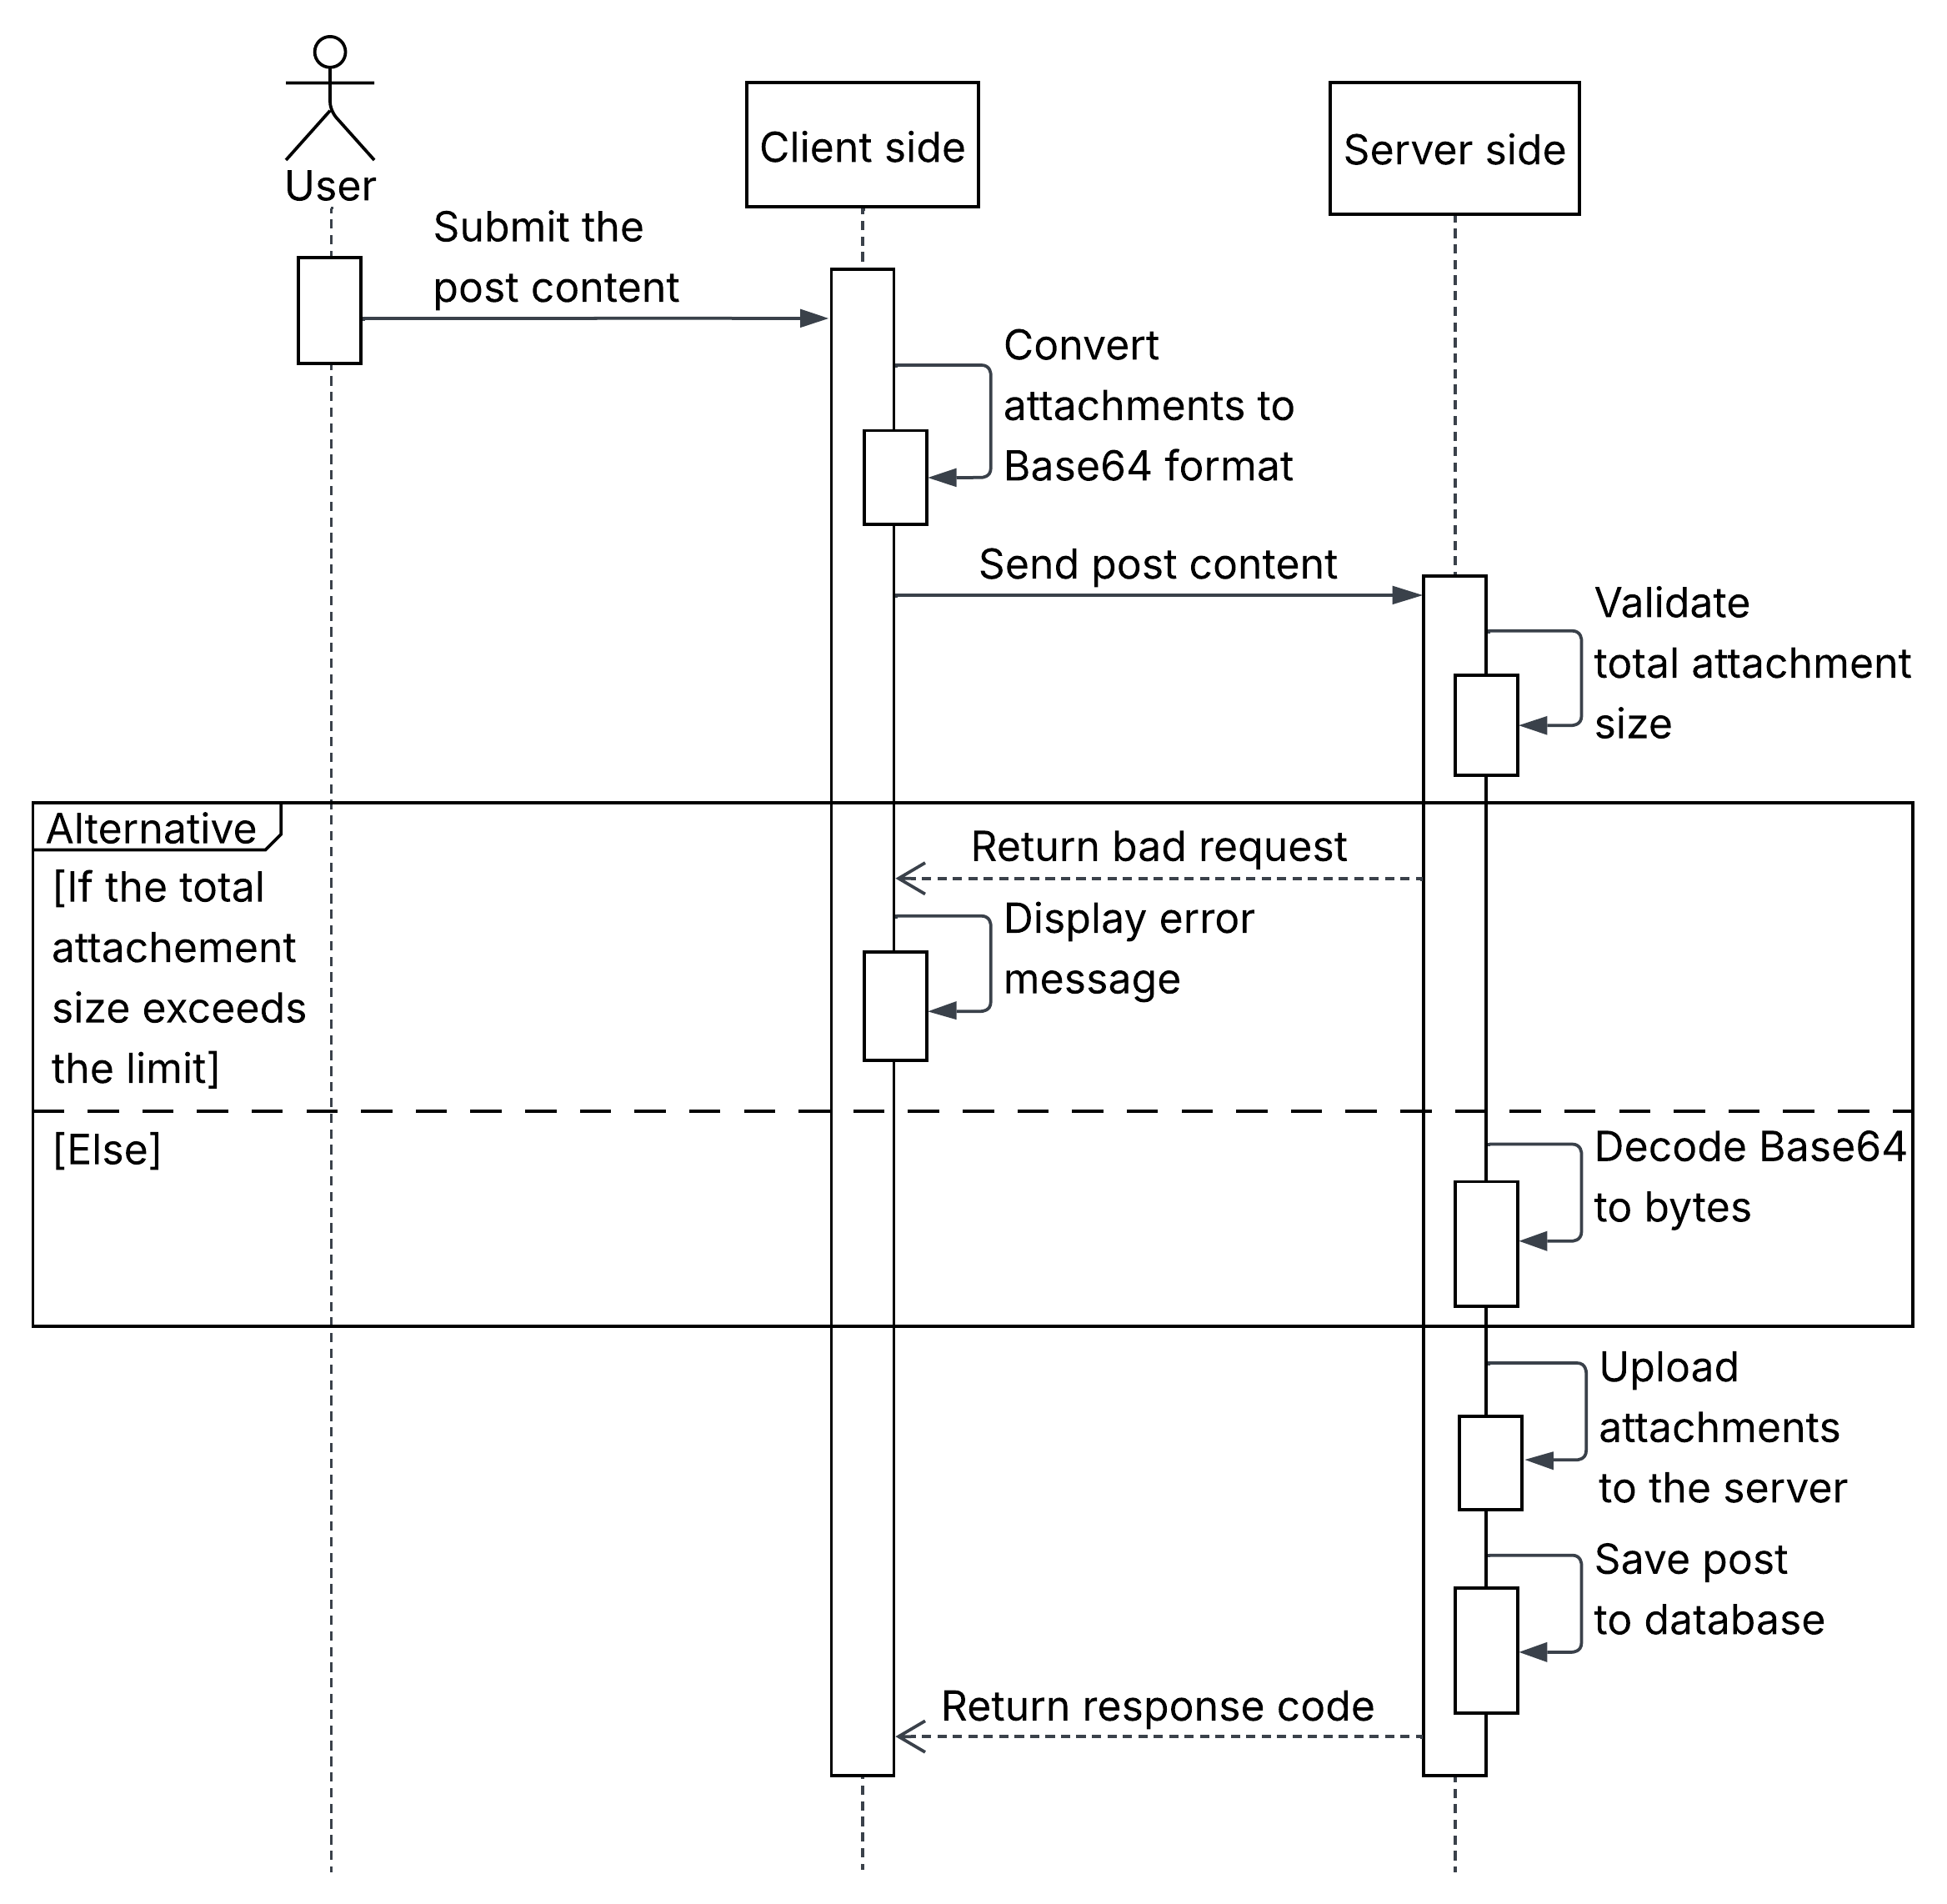
\includegraphics[width=1\textwidth]{images/sqd_post_newsfeed.png}
    \vspace{-1em}
    \caption{Post newsfeed sequence diagram.}
    \label{fig:sequence_diagram_post_newsfeed}
\end{figure}
\begin{minipage}{\textwidth}
    \setlength{\parindent}{2em}
    The sequence diagram illustrates the flow of actions when a teacher posts a newsfeed to the class. When a teacher creates a newsfeed post, the client-side application processes the content and converts any attachments to base64 format for transmission. After that, the system receives a request from the client side and validates the post. If the total attachment size does not exceed the limit, the system decodes the attachments to bytes, uploads the attachments to the server storage, and saves the post content to the database. Once processing is complete, the post is created and all student parents can view and interact with the post, enabling them to stay informed about their child's classroom and school activities.
\end{minipage}

% TRACK BUSES
\subsubsection{Sequence Diagram for Track Buses}
\vspace{-1.5em}
\begin{figure}[H]
    \centering
    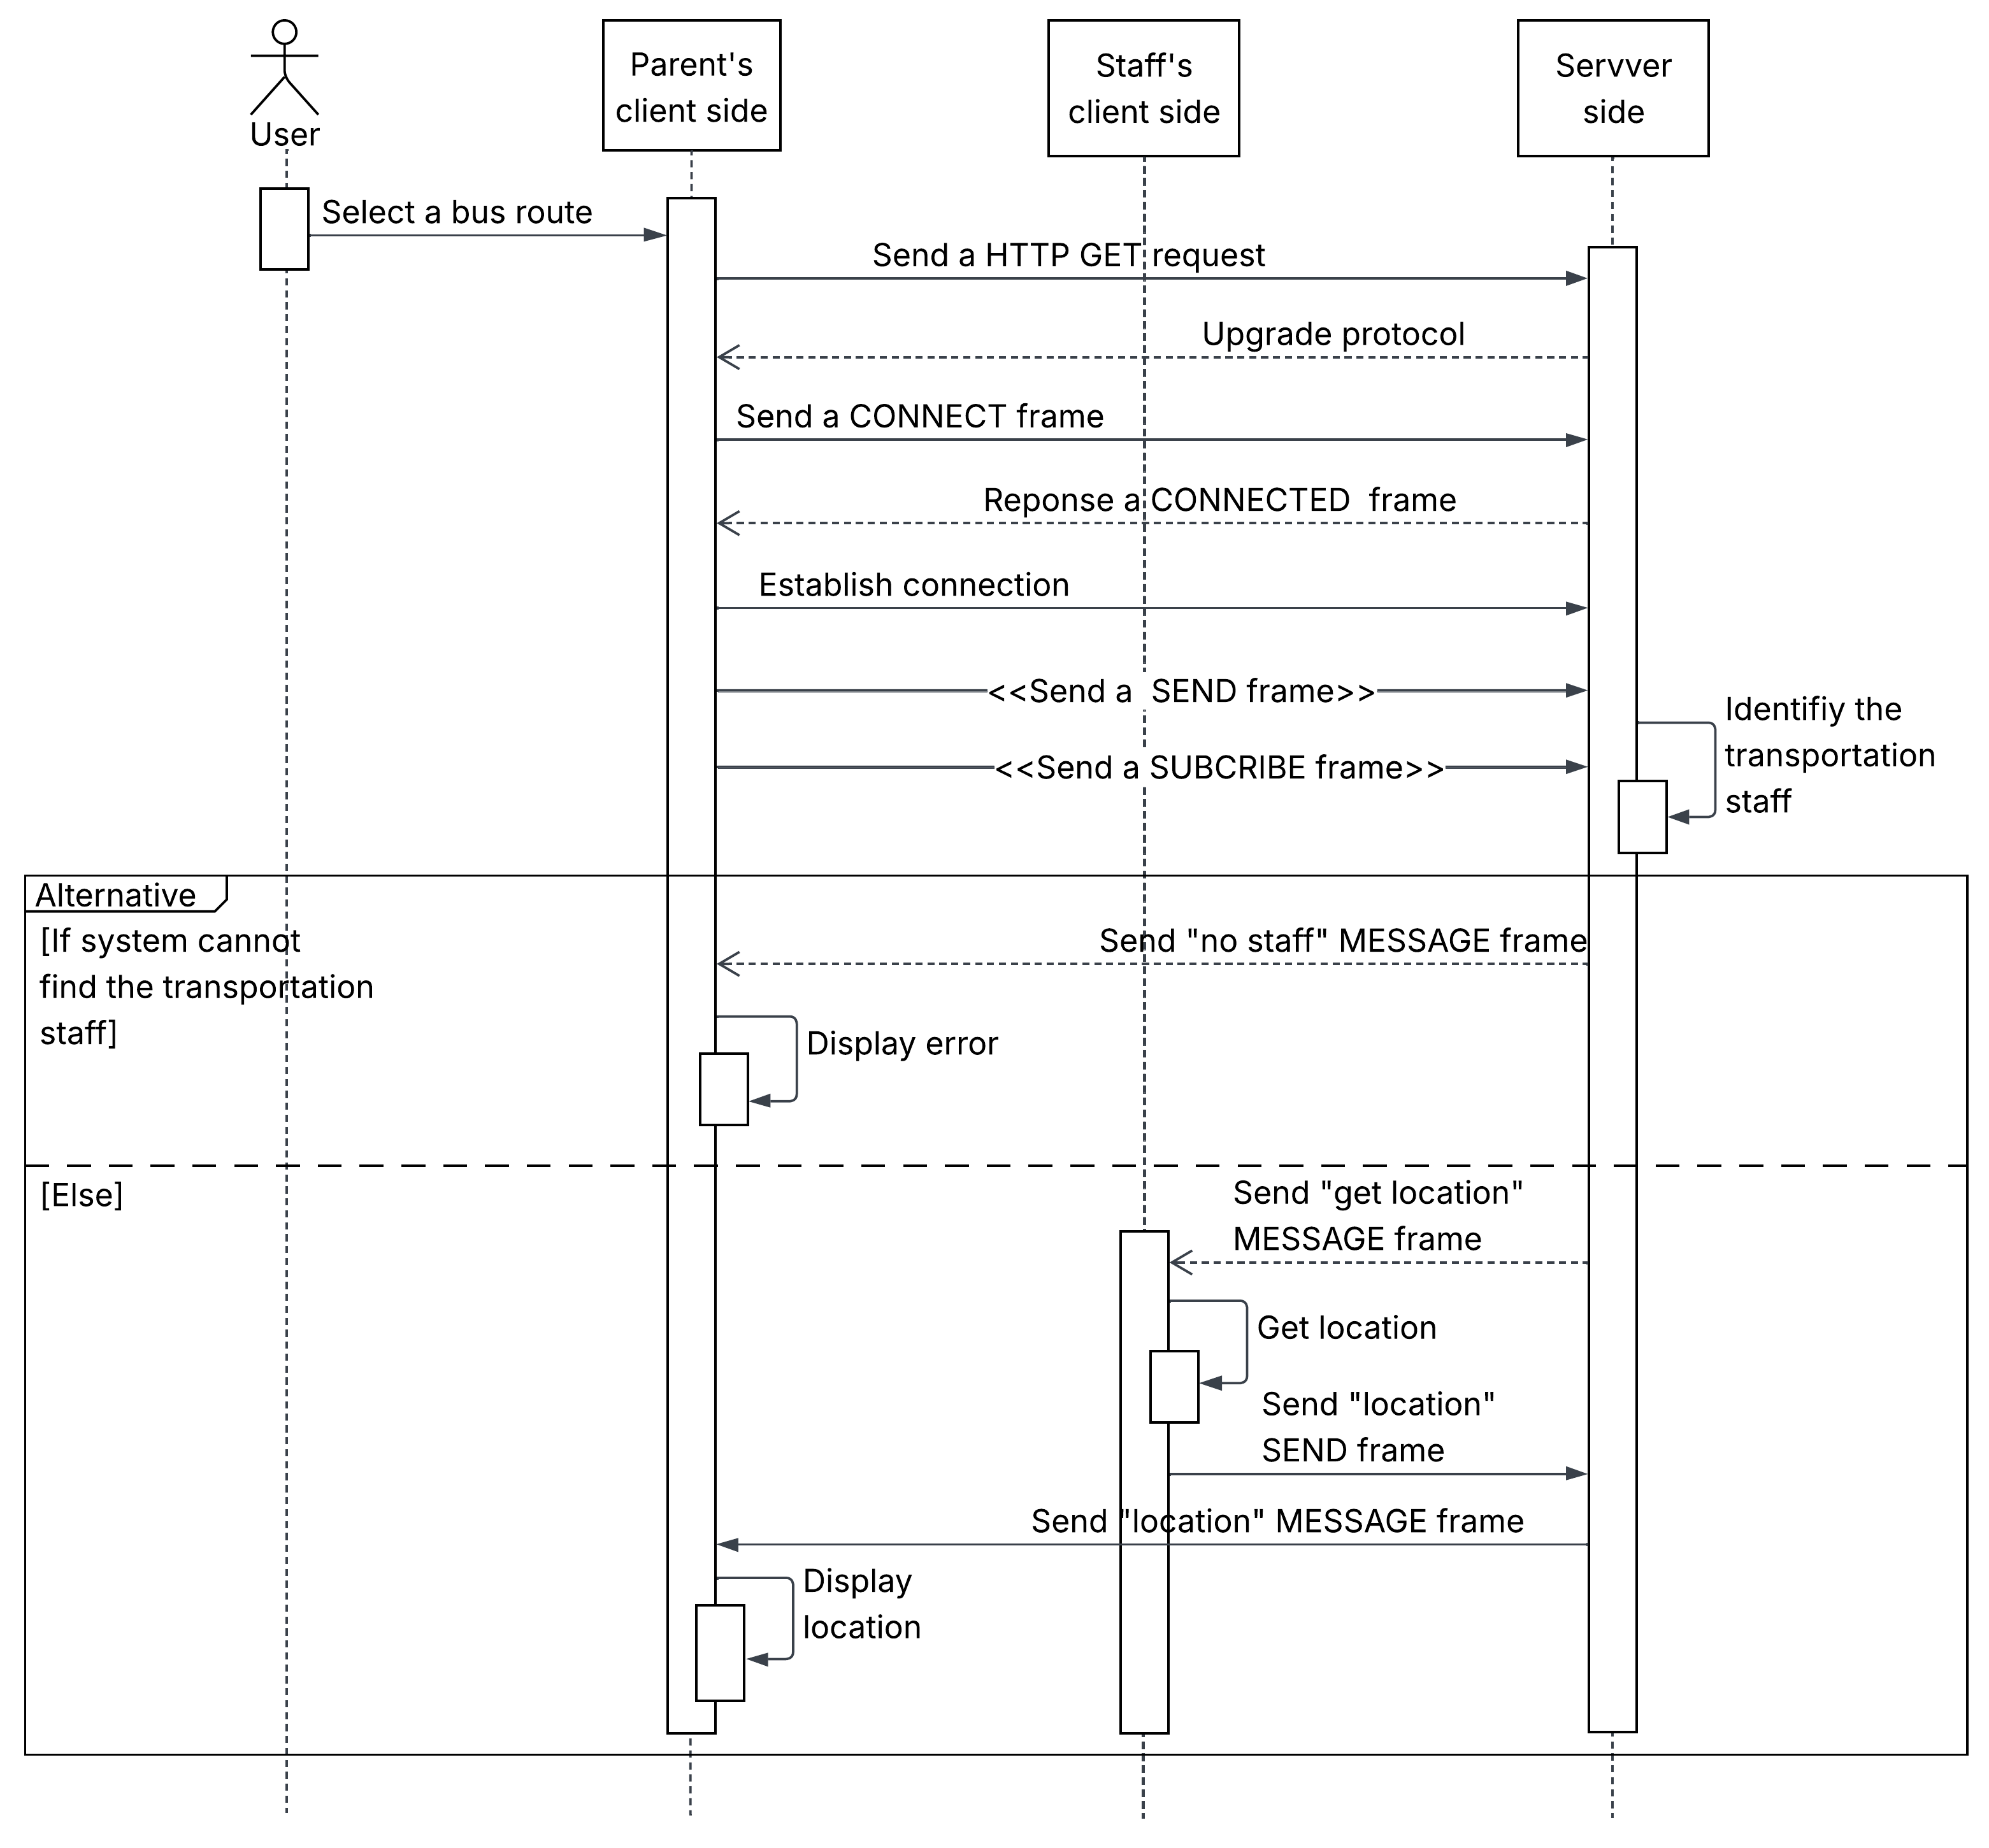
\includegraphics[width=1\textwidth]{images/sqd_track_bus.png}
    \vspace{-1em}
    \caption{Track buses sequence diagram.}
    \label{fig:sequence_diagram_track_buses}
\end{figure}
\begin{minipage}{\textwidth}
    \setlength{\parindent}{2em}
    The sequence diagram illustrates the real-time bus tracking process that enables parents to monitor their children's school buses. The workflow begins when a parent selects a specific bus route, prompting the client to initiate a WebSocket connection via an HTTP GET request, followed by a STOMP CONNECT frame. Once connected, the parent's client side sends a SEND frame to request the transportation staff location and a SUBSCRIBE frame to receive live updates. The system checks if transportation staff is assigned to the selected route. If available, the server sends a MESSAGE frame to the staff, prompting them to share their location. The staff client then sends location updates every 50 meters via SEND frames, which the server broadcasts to all subscribed parents. If no staff is assigned, the system notifies the parent immediately.
\end{minipage}